\subsection{Profile Composition, Specific Members, and Retained Subgroups}
\label{sec:composition}
\subsubsection{Profile proportions shift averages; member choices retain a wide spread}
\label{sec:composition-discussion-anchor}

Increasing the proportion of turn-retaining (C3) annotators systematically raises average team quality, yet teams sharing the exact same profile counts still span a wide performance range depending on which specific individuals are selected. In 12-person teams, increasing the C3 count by one while decreasing the C2 count by one raises mean $Q$ across the member sets in each composition by 1.969 points across 37 panoramas (increasing on 31 of 37). However, within any fixed profile composition, the mean fifth-to-95th percentile spread across distinct member combinations reaches 24.091 $Q$ points on difficult panoramas and 6.037 points on easy panoramas (Figure~\ref{fig:composition-members}). In panel (a), moving from left to right shifts the composition counts from C2 to C3 while the C1 count remains fixed. Mean Q rises, but the broad fifth-to-95th percentile ranges show that specific member choices still produce substantially different outcomes within the same composition.

\begin{figure*}[t]
\centering
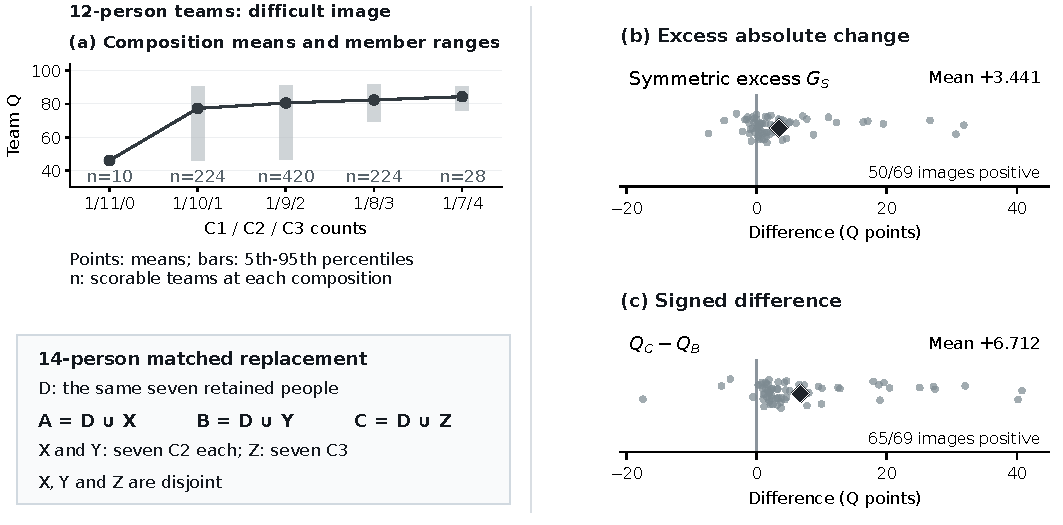
\includegraphics[width=145mm]{figures/composition_replacement_rev11.pdf}
\caption{Composition summaries and specified replacements reveal different aspects of member sensitivity. (a) Twelve-person teams on zsNo4HB9uLZ-16 combine six fixed members with six of twelve candidates. Horizontal labels give C1/C2/C3 member counts; points are mean Q, bars show fifth--95th percentiles, and $n$ gives the number of scorable teams. (b--c) A separate 14-person A--B--C comparison shares seven retained members and exchanges seven-person blocks. (b) Excess magnitude $G_S$ compares cross-profile and within-profile Q changes; (c) signed $Q_C-Q_B$ shows whether C scores higher or lower than B. Each dot is an image mean; diamonds average the 69 image means from 146 scorable events (comparison definitions and supporting results in Supplements C17 and C19).}
\label{fig:composition-members}
\label{fig:matched-half}
\label{fig:team-comparison-design}
\end{figure*}

Across 231 panels (40 panoramas in 22 buildings), we enumerate all 924 ways to select six of twelve candidates and combine them with a background fixed within each panel. Backgrounds contain 6--23 people, producing teams of 12--29; Figure~\ref{fig:composition-members} illustrates a 12-person panel. This enumeration quantifies the balance between profile composition and member choice: under the C1--C3 profile partition, differences between profile compositions account for 15.43\% of the total $Q$ variance, whereas differences among specific member sets within the same composition account for the remaining 84.57\% (weighted by scorable teams within compositions and equally across buildings; Supplement C17). Profile proportions describe mean trends, while member combinations within the same proportions account for most of the variation in these enumerated teams.

Different profile families also expose distinct quality--labor trade-offs. On their respective shared supports in 12-person teams, the one-seat C2-to-C3 composition contrast raises mean $Q$ by 1.963 points with a recorded labor ratio of 1.020 across 27 panoramas. The corresponding J3-to-J4 contrast (ordered by increasing training-fold $Q$ residuals) raises mean $Q$ by 2.701 points with a labor ratio of 0.897 across 14 panoramas. Similarly, historical consensus-response profiles (R1--R2) directly track individual impact on group geometry: R2 annotators outscore R1 annotators by 13.937 individual-$Q$ points across 192 shared panoramas, and cross-profile swaps between R1 and R2 induce larger consensus shifts than within-profile swaps on 62 of 83 panoramas (Supplement C19).

\subsubsection{Within-profile and cross-profile replacements}

Controlled block replacements reveal both the greater magnitude of cross-profile changes and their quality direction: C2-to-C3 exchanges usually raise $Q$, while matched within-profile alternatives establish how much change also occurs when the class is held fixed. In direct A--C comparisons on 14-person teams, replacing a seven-person C2 block with a C3 block (while holding the seven background members fixed) increases team $Q$ by an average of 6.190 points, with positive gains on 77 of 83 panoramas. Adding a matched within-profile control block $B$ in our A--B--C design---where teams $A$ and $B$ add disjoint C2 blocks and team $C$ adds a C3 block to the same seven-person background---shows that cross-profile replacement exceeds within-profile variation by a mean symmetric excess of $G_S = 3.441$ points across 69 jointly scorable panoramas (positive on 50), with team $C$ outscoring team $B$ by $\Delta_{CB} = 6.712$ points (positive on 65; Figure~\ref{fig:matched-half}).

The six-person C1--C3 comparisons sharpen this distinction: cross-profile exchanges produce larger changes in both directions, while reversing the exchange reverses the mean quality effect. In six-person teams, exchanging three members between C1 and C3 across 36 shared panoramas yields mean excess magnitudes of $G_S = 3.269$ (C1-to-C3) and $3.955$ (C3-to-C1), accompanied by signed effects of $\Delta_{CB} = +7.327$ and $-7.777$ $Q$ points, respectively (Supplement C19). In 20-person teams, a seven-person C2-to-C3 replacement increases $Q$ by 4.484 points across 84 panoramas; on the 40 panoramas with shared quality and timing records, $Q$ rises by 4.406 points while total team labor increases by 121.05 person-seconds.

Combining entire profile classes into whole-profile mixtures reveals how incoming votes can either recover missed features or dilute intricate detail. Across 154 shared panoramas in 22 buildings, pooling all available C2 and C3 annotators (C2+C3) expands the team as well as changing its composition, yielding a mean $Q$ of 88.52---outperforming pure C2 teams (84.83) but falling below pure C3 teams (92.29; Figure~\ref{fig:profile-mixtures}). The dilution is sharpest on complex geometry: across 34 difficult panoramas, the C2+C3 mixture scores 19.768 points below pure C3 (losing on 26 panoramas), and across 36 self-occluded panoramas it retains 2.389 fewer turns and 1.389 fewer short edges, alongside an 18.467-point drop in $Q$. When incoming members omit a fine wall turn, their addition can raise the at-least-half threshold beyond its existing support, removing a recess retained by the smaller team (as illustrated in Figure~\ref{fig:bathroom-turn-votes}).

\begin{figure}[t]
\centering
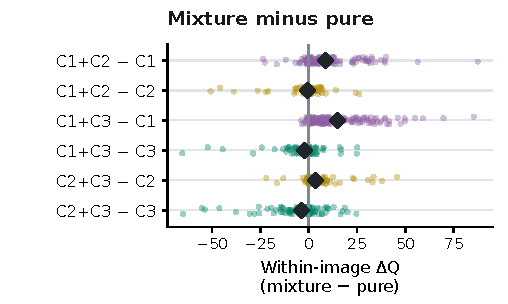
\includegraphics[width=86mm]{figures/profile_mixtures_rev11.pdf}
\caption{Whole-profile mixtures gain relative to one constituent and lose relative to another. Dots are paired image-level mixture-minus-pure Q differences on 154 common images; diamonds are means. Each selected profile contributes all its available members.}
\label{fig:profile-mixtures}
\end{figure}

\subsubsection{Retained people alter replacement direction and boundary position}

The impact of a member replacement depends not only on who is swapped, but also on the retained background $D$. In the joint-profile comparison, expanding the retained background reduces the average magnitude of a fixed exchange: holding seven-person replacement blocks constant while increasing total team size from 20 to 28 reduces the mean absolute $Q$ shift by 1.317 points across 76 panoramas (shrinking on 63). More strikingly, rotating the retained background members can reverse the sign of the exact same exchange. Among 276 replacement blocks evaluated across at least two scorable backgrounds, 56 blocks (20.3\%, spanning seven panoramas) produced both positive and negative $Q$ shifts, with 24 blocks crossing both $+1$ and $-1$ $Q$ points. Even when holding the background's profile counts strictly fixed, 18 of 120 subgroups reversed direction, including nine that crossed both $\pm 1$-point thresholds (Supplement C19).

A concrete 14-person comparison on panorama \texttt{q9vSo1VnCiC-30} illustrates how specific retained members dictate the effect of incoming observations. Two distinct seven-person backgrounds each contained exactly one C1 and six C2 annotators; yet applying the identical seven-person C2-to-C3 replacement reduced $Q$ from 85.130 to 81.090 under the first background while boosting $Q$ from 38.146 to 87.269 under the second, because the two backgrounds anchored the consensus around different initial structures and boundary positions.

Furthermore, member replacements reshape boundary localization even when the corner count remains unchanged; the illustrated case also preserves the corner identities and their ring order. Among 1,829 jointly scorable 20-person replacement pairs, 1,632 retained the exact same number of corners, yet 127 of those constant-count pairs shifted by more than 10 $Q$ points. In panorama \texttt{7y3sRwLe3Va-13} (Figure~\ref{fig:localization-mechanism}), all four room corners retain unanimous 20-vote support and identical cyclic ordering before and after a seven-person swap, yet the new members' endpoint coordinates shift the median consensus positions enough to raise $Q$ from 77.41 to 92.58.

\begin{figure*}[t]
\centering
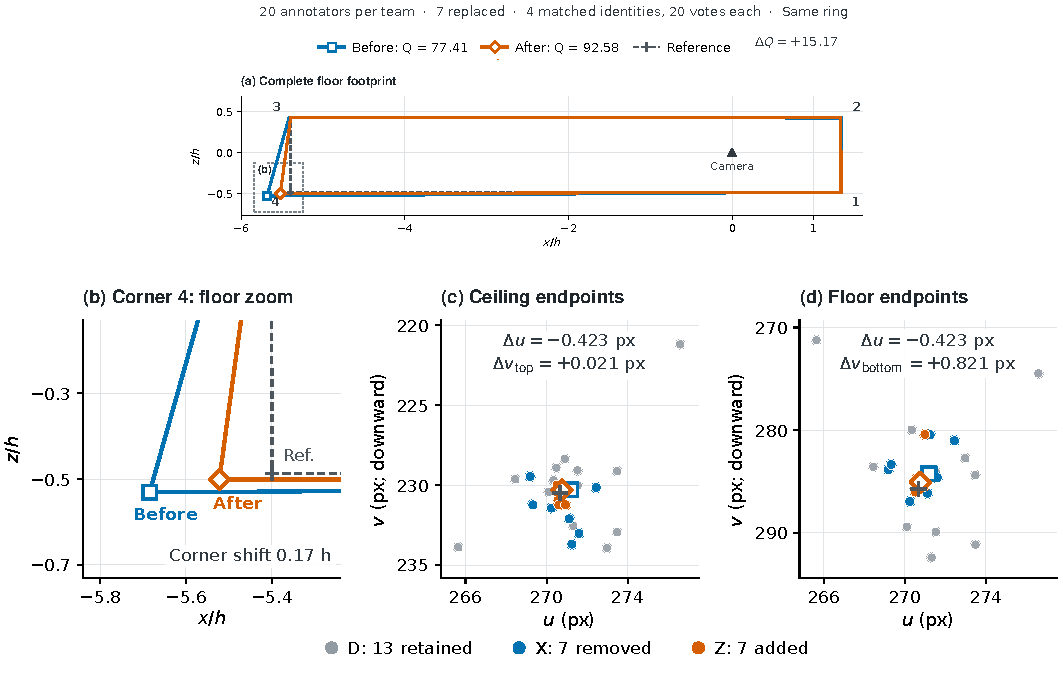
\includegraphics[width=115mm]{figures/localization_compact2.pdf}
\caption{Seven replacements change localization while four identities retain twenty votes and the same ring order in 7y3sRwLe3Va-13. Panels show the complete footprints, corner-4 detail and its upper/lower observations. Gray marks thirteen retained people, blue seven removed and orange seven added; outlined markers are consensus positions. Changes of about 0.42 horizontal and 0.82 lower-endpoint pixels correspond to a floor displacement of $0.17h$ in the 1024 by 512 panorama. Q measures the complete layout.}
\label{fig:localization-mechanism}
\end{figure*}

Decomposing $Q$ into its five geometric components further explains why 7 of 84 panoramas in the 20-person C2-to-C3 exchange gained prism IoU while losing $Q$: on \texttt{x8F5xyUWy9e-03}, for example, $Q$ dropped by 4.726 points as internal directional error rose by $0.836^\circ$ alongside local boundary and height shifts (Supplement C19).


